\section{Out-of-Time-Order Correlator in~integrable~systems with local hyperbolicity}%
\label{sec:OTOC_theory}%
Our goal in this section is to refine the pre-Ehrenfest theory for scrambling around hyperbolic fixed points in integrable systems. In particular we attempt to relax the localization properties of the initial state considered in~\cite{Hummel2019,Scaffidi2020}.
%
The OTOC for two operators $\hat{A}$, $\hat{B}$ with respect to a state $\hat{\rho}$ is defined by 
\begin{align}
    \mathbf{ C}(t) \,=\, \operatorname{tr} \big\{\hat{\rho} \big| [\hat{A}(t),\hat{B} ] \big|^2 \big\},
    \label{eq:OTOC_def} 
\end{align}
which is by itself a modulus-squared commutator. When this squared commutator is expanded in individual correlators one obtains, besides contributions that admit a standard time ordering, extra irreducibly un-ordered correlations \cite{Maldacena_2016}, with anomalous dynamical behavior that are the central object of study.  

The long-time~(post-Ehrenfest) saturation of generic OTOCs has been subject of several studies, both in the chaotic \cite{Josef2018,argentinians} and integrable \cite{Hummel2019,Fortes} regimes where interference effects beyond a pure quasiclassical (Truncated-Wigner like-) approach appear~\cite{Polkovnikov2011}.

Here, however, our focus is the short time scales, where a quasiclassical approach based on the Wigner-Moyal expansion, which is a regular expansion around $\hbarE=0$ \cite{schleich01,Kim1991,connell2008}, is perfectly appropriate. Keeping only leading-order terms in $\hbarE$, one obtains %(see App.~\ref{sec:appendixWignerMoyal})\rc{maybe an appendix? YES but not in present arXiv version, just put as reference the quantum optics in phase space book}

    \begin{align}
        \begin{split}
            \mathbf{ C}(t) \,=\,& \hbarE^{2} \langle W_{\rho}(\Vec{q}_{0},\Vec{p}_{0}) \big|\big\{ A_{\rm W}(\Vec{q}_{0},\Vec{p}_{0},t), B_{\rm W}(\Vec{q}_{0},\Vec{p}_{0}) \big\}  \big|^{2}\rangle_{\text{PS}}
            \\
            &+ O(\hbarE^{4}),
        \end{split}
         \label{eq:WignerWeyl}
    \end{align}
    where $A_{W}$, $B_{W}$ are the Wigner-transforms of the operators $\hat{A},\hat{B}$ and $W_{\rho}(\Vec{q}_{0},\Vec{p}_{0})$   is the Wigner-distribution corresponding to the state $\hat{\rho}$. 

    
    Further, $\langle  . \rangle_{\text{PS}}$ indicates integration over the whole classical (mean-field) phase space parametrized by the canonical pairs $(\Vec{q}_{0},\Vec{p}_{0})$. The Heisenberg time dynamics of the quantum operator is mapped to time dynamics of the classical observable $A(q_{0},p_{0},t) =A(q(q_{0},p_{0},t),p(q_{0},p_{0},t)) $ which arises from the classical propagation of the initial values $q_{0}$ and $p_{0}$.
    
    The effective Plank constant $\hbarE$ has different expressions in different contexts. It is given by the usual Plank constant divided a typical action $\hbar/S_{\rm typ}$ in single particle cases \cite{Gutzwiller1991,Haake2001,brack1997}, and the inverse of the total spin quantum number $1/S$ for spin systems \cite{Waltner2017PRL,Waltner2020PRE}. In the case of interest here, interacting bosonic systems, $\hbarE = \frac{1}{N}$  is given by the inverse of the total particle number $N$ after convenient rescaling of the interaction strength \cite{Richter2022,Engl2015PRE}.
    
    Without loss of generality, we choose the operators $\hat{A}=\hat{q}$ and $\hat{B}=\hat{p}$, as they are hermitian and their classical counterparts are generalized coordinates or momenta. Therefore, at leading order in the Wigner-Moyal expansion, Eq.~\eqref{eq:WignerWeyl},
    we drop the index ${}_W$ and take the pure classical phase space functions. This choice of the operators simplifies the classical Poisson-brackets, that are now given by an element of the stability matrix $\frac{\partial \vec{x}(t)}{\partial \vec{x}(0)}$ with $\vec{x} = (\vec{q},\vec{p})$ \cite{tabor1989chaos,wiggins2003}. 

    The classical limit of the OTOC in Eq.~(\ref{eq:WignerWeyl}) is so far a completely general result. Under the assumption of local instability, however, the leading order of exponential growth is given by the maximal local exponent $\lambda(\vec{q}_{0},\vec{p}_{0})$ of the stability matrix:
    \begin{align}
         \mathbf{ C}(t) ~\sim~& \hbarE^{2} \langle W_{\rho}(\Vec{q}_{0},\Vec{p}_{0}) \exp\big\{ 2 \lambda(\Vec{q}_{0},\Vec{p}_{0}) t\big\}  \rangle_{\text{PS}}.
         \label{eq:WignerWeylFP}
    \end{align}
    
    At this point, it is convenient to introduce two local time-scales:
    \begin{itemize}
        \item After the local ergodic time $\tLoc= 1/\lambda (\Vec{q}_{0},\Vec{p}_{0})$,  the exponential growth of the OTOC begins to be visible. Before $\tLoc$, we have sub-exponential/polynomial behavior linked to system-specific mechanisms.
        \item The Wigner-Weyl approximation breaks down when the leading order of the integrand in Eq.~\eqref{eq:WignerWeyl} becomes large compared to $\hbarE^{2}$. This breakdown defines the local Ehrenfest time $\tEhr= \lambda^{-1}(\Vec{q}_{0},\Vec{p}_{0})  \log (1/\hbarE)$ and in our many-body case $\tEhr= \lambda^{-1}(\Vec{q}_{0},\Vec{p}_{0}) \log N$.
    \end{itemize}
    
    We exploit the experimentally tunable localization features of quantum mechanical states \cite{squeezingBEC2008} as a tool to probe the local unstable dynamics around a hyperbolic fixed point (FP)  and consider a coherent-like state~$\hat{\rho}$  centered around it. 
    In the linearized region around the FP the dynamics can be precisely described, and we can express $\lambda(\vec{q}_{0},\vec{p}_{0})$ by the maximal stability exponent $\ls$ of the FP. 
    In general, however, the linearized region is bounded and we express this by the fact that the relation $\{ A(\vec{q}_{0},\vec{p}_{0},t), B(\vec{q}_{0},\vec{p}_{0})\} = e^{\ls t} $ is valid only if the unstable manifold coordinate/projection $u(\vec{q}_{0}$, $\vec{p}_{0})$ is smaller than a threshold $c>0$. 
    For times larger than zero, the exponential growth $u(\vec{q}_{0},\vec{p}_{0},t)= u(\vec{q}_{0},\vec{p}_{0}) e^{\ls t}$ is only valid if the linearized region $u(\vec{q}(t),\vec{p}(t),t)< c$ is still fulfilled. Afterwards we need to replace the time dynamics of the unstable manifold by a sub-exponential function. We refer to this mechanism as a kind of {\it leaking} from the linearized region \cite{Scaffidi2020}.%\rc{(cite Scaffidi)}
    
    The key observation is that, although the sub-exponential function describes the classical evolution outside and it is therefore negligibly  small compared to the exponential growth in the linearized region, its contribution is weighted by a portion of phase space that grows exponentially. These considerations allow us to heuristically account for the leaking mechanism, by modifying the Eq. \eqref{eq:WignerWeylFP} as
    \begin{align}
         \mathbf{ C}(t) ~\sim~& \hbarE^{2} e^{ 2 \ls t} \langle W_{\rho}(\Vec{q}_{0},\Vec{p}_{0}) \Theta ( c - e^{\ls t} u(\vec{q}_{0}, \vec{p}_{0}))\rangle_{\text{LR}},
         \label{eq:WignerWeylFPLeaking}
    \end{align}
    where we restrict the phase-space integration to the dominant linearized region (LR) around the FP.

    For definiteness, let us consider now a Gaussian wave-packet with an initial linear width  $\Delta u$ along the unstable manifold $u(\vec{q},\vec{p})$.
    %Leaking affects the dynamics of the OTOC \ref{eq:WignerWeyl} for a wave-packet with an initial linear width $\Delta u$ along the unstable manifold $u(\vec{q},\vec{p})$.
    In this situation, the wave-packet reaches the boundary of the  linear region by a finite time $\tLeak = \ls^{-1} \log \big( c/\Delta u \big)$, which we correspondingly call the leaking time. 
    After $\tLeak$, we must take the leaking of the wave-packet into account, i.e., the phase-space volume causing the exponential growth shrinks exponentially with $e^{-\ls t}$, i.e.,
    \begin{align*}
        \langle W_{\rho}(\Vec{q}_{0},\Vec{p}_{0}) \Theta ( c - e^{\ls t} u(\vec{q}_{0}, \vec{p}_{0}))\rangle_{\text{LR}} \,\sim \,
        \left\{\begin{array}{ll}
            \text{const.} &,t<\tLeak \\
            e^{-\ls t} &,t>\tLeak \\
             \end{array}\right. \! .
    \end{align*}
    Hence, the exponential growth of the OTOC in Eq. \eqref{eq:WignerWeylFPLeaking} decreases to $e^{\ls t}$. 
    This finally leads to a short-time behavior of the OTOC around an unstable fixed point given by
    \begin{align}
        \mathbf{ C }(t)~\sim~
            \left\{\begin{array}{ll}
            \text{poly.} & ,t<\tLoc \\
             e^{2\ls t}& ,\tLoc<t<\tLeak\\
             e^{\ls t} & ,\tLeak<t<\tEhr\\
             \text{osc.} & ,\tEhr < t 
             \end{array}\right.
             ,
             \label{eq:OverviewFP}
    \end{align}
     that is schematically displayed in Fig. \ref{fig:SchematicOTOC_FP} showing two exponential regions. 
    \begin{figure}[h!]
        \centering
        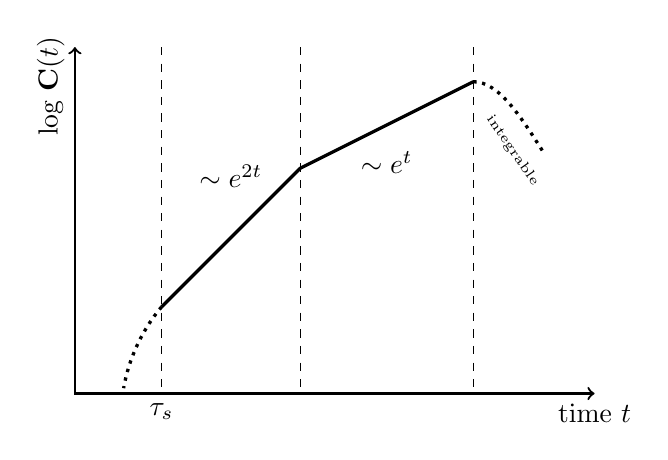
\begin{tikzpicture}[scale=2.2]
            % Draw axes
            \draw [<->,thick] (0,2) node (yaxis) [above,rotate=90,xshift=-0.5cm] {log $\mathbf{C}(t)$}
                |- (3,0) node (xaxis) [below] {time $t$};
            \draw[dashed] (0.5,2) -- (0.5,0) node[below] {$\tau_{s}$};
            \draw[dashed] (1.3,2) -- (1.3,0)  node[below] {$\tLeak$};
            \draw[dashed] (2.3,2) -- (2.3,0) node[below] {$\tEhr$};
            \draw[very thick] (0.5,0.5) -- (1.3,1.3)node [midway, above,yshift=0.5cm] {$\sim e^{2\ls t}$} -- (2.3,1.8) node [midway, below,yshift=-0.2cm] {$\sim e^{\ls t}$};
            \draw[very thick, dotted] (0.5,0.5) arc[start angle=140, end angle=170,radius=1cm] ;
            %\draw[very thick, dotted] (2.3,1.8) -- (2.9,1.8) node[midway,above] {\tiny chaotic};
            \draw[very thick, dotted] (2.3,1.8) cos (2.7,1.4);
            \draw  (2.45,1.35) node[above,rotate=-55.5] {\tiny integrable};
        \end{tikzpicture}        
        \caption{Expected behavior of an OTOC centered at a FP if~$\tLoc<\tLeak< \tEhr$: OTOCs grow polynomial for times shorter $\tLoc$, exponential with $2\ls$ for times shorter $\tLeak$, exponential with $\ls $ for times shorter $\tEhr$, but greater than $\tLeak$. Post-Ehrenfest time scales display oscillatory behaviour if the system is integrable~\cite{Fortes} and saturation if the system is chaotic \cite{Josef2018,PhysRevE.98.062218}. }
        \label{fig:SchematicOTOC_FP}
    \end{figure}
    
    It is important to note that there is a hierarchy of time scales: the leaking time is only relevant if~$\tLeak < \tEhr$, otherwise the Wigner-Weyl approximation (in leading order), see Eq.~\eqref{eq:WignerWeyl}, is already invalid. 

    The initial linear width $\Delta u$ scales with some power $\hbar_{\rm eff}^{\alpha}$ for typical states. This gives an asymptotic expression for the leaking time by $\tLeak\sim \frac{\alpha}{ \ls} \log N + O(\log(c))$. Hence, we have a direct proportional relation to the Ehrenfest time $ \tLeak \sim  \alpha\tEhr$ for $\hbarE\to 0$.
    
    We see then, that one can clearly distinguish three parametric regions: $\tLeak < \tLoc$,  $\tLoc<\tLeak < \tEhr$ and $\tEhr \leq \tLeak$ (which is equivalent to $\alpha\approx 0,<1,\approx 1$):
    \begin{enumerate}[label=\roman*)]
        \item Delocalized/uniform states: $\tLeak < \tLoc$, $\alpha\approx 0$\\
        We need to assume the FP we chose is the only unstable FP of the classical dynamics.
        Then, the OTOC is still governed by Eq.~\eqref{eq:OverviewFP} and the $e^{2\ls t}$-regime vanishes. 
        A    typical examples here are high temperature states ($T\to \infty$).
        \item Localized states:  $\tLoc<\tLeak < \tEhr$, $0< \alpha <1$\\
            In this case we have the $2\ls -\ls$ transition and asymptotically (for $N\to \infty$) we expect a sharp kink to appear at $\tLeak$.
           The prime example are the coherent states centered at a FP. They usually have a linear size of $\hbarE^{1/2}$ in all phase space directions. 
        \item Well-localized states: $\tLeak\approx \tEhr$, $\alpha \approx 1$\\
            The second $e^{\ls t}$-region is vanishing, only the one $e^{2\ls t}$-region is visible. 
            Fock states are candidates for the third class. Their linear width is $\hbarE$ in the classical occupation numbers, such that $\alpha \approx 1$ if the unstable manifold is aligned in the parallel direction.  
    \end{enumerate}
The case $\alpha>1$ is unphysical and can be excluded. The uncertainty principle requires the product of the width in all directions to be $\geq \frac{\hbarE}{2}$. Hence if $\alpha>1$, one direction must increase if $\hbarE\to 0$, i.e., this direction becomes delocalized if we approach the classical limit contradicting that the state is associated by a well-defined point in phase space. %Delocalization contradicts such a classical limit.% \rc{maybe explain why? I mean... a Fock state is delocalized and admits a classical limit in the sense of an ensemble...}.

At this point, we can explain the dynamical behavior of OTOCs reported in \cite{Hummel2019} and \cite{Scaffidi2020}. In the first paper, the authors investigated a number-projected coherent state which is simultaneously a Fock state. Its unstable manifold is parallel to the occupation direction \cite{thesisBenni}, therefore it falls into the case  iii) and they see only the $2\ls$-exponential window. Correspondingly, the authors of the second paper  use the infinite temperature state, hence their state directly falls into the first case and the only exponential window is given by $e^{\ls t}$.

In the next section, we numerically explore the validity Eq. \eqref{eq:OverviewFP} for a  Bose-Hubbard dimer, with the aim of carefully investigate the new case  ii), where the hierarchy of time scales $\tLoc<\tLeak<\tEhr$ implies, from our analysis, the presence of a $2\ls-\ls$ transition.